\chapter{Experiment}
\label{ch:Experiment}

\section{Environment}
The experiment was conducted on the Raspberry Pi 4 Model B. 
The Pi's computational capabilities are powered by a Broadcom BCM2711 chip \cite{bcm2711-arm}
consisting of four Cortex-A72 processing cores, each having a 48 kB and 32 kB L1 instruction 
and data cache, respectively. The local caches are connected to a central 1 MB L2 cache, which is also 
used by an integrated VideoCore 6 GPU. The SoC interfaces with an 8 GB LPDDR4-SDRAM chip through a 
32-bit wide bus. A 64 GB SanDisk microSD card is used for persistent storage.

\begin{figure}[H]
    \centering
    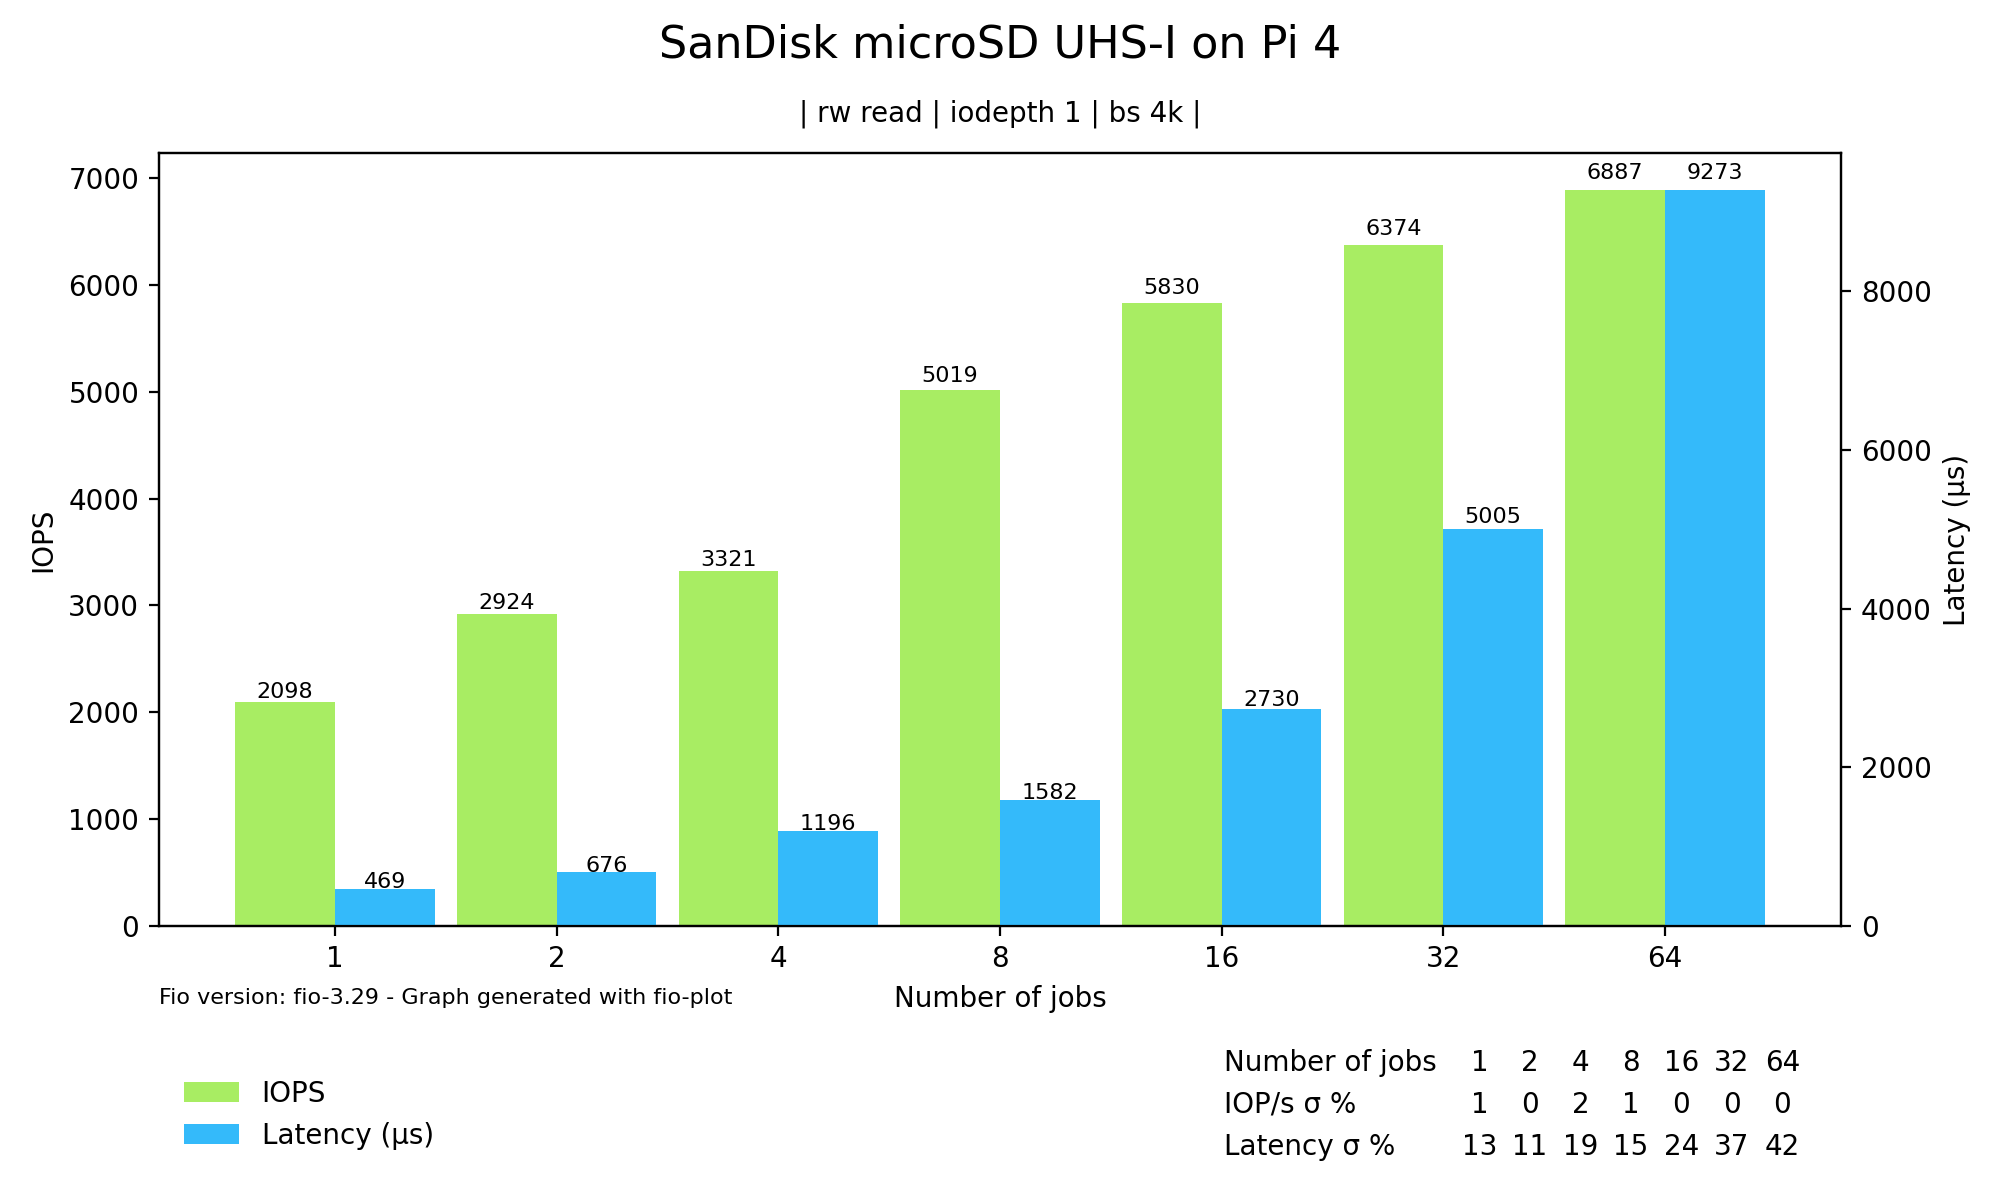
\includegraphics[width=0.8\textwidth]{images/results/sandisk-host-libaio-read-numjobs-iops-latency.png}
    \caption{Throughput and latency measurements on the host as a function of the number of concurrent processes issuing asynchronous reads.}
    \label{images:fundamentals/net-ns-veth-arch.jpg}
\end{figure}

\begin{figure}[H]
    \centering
    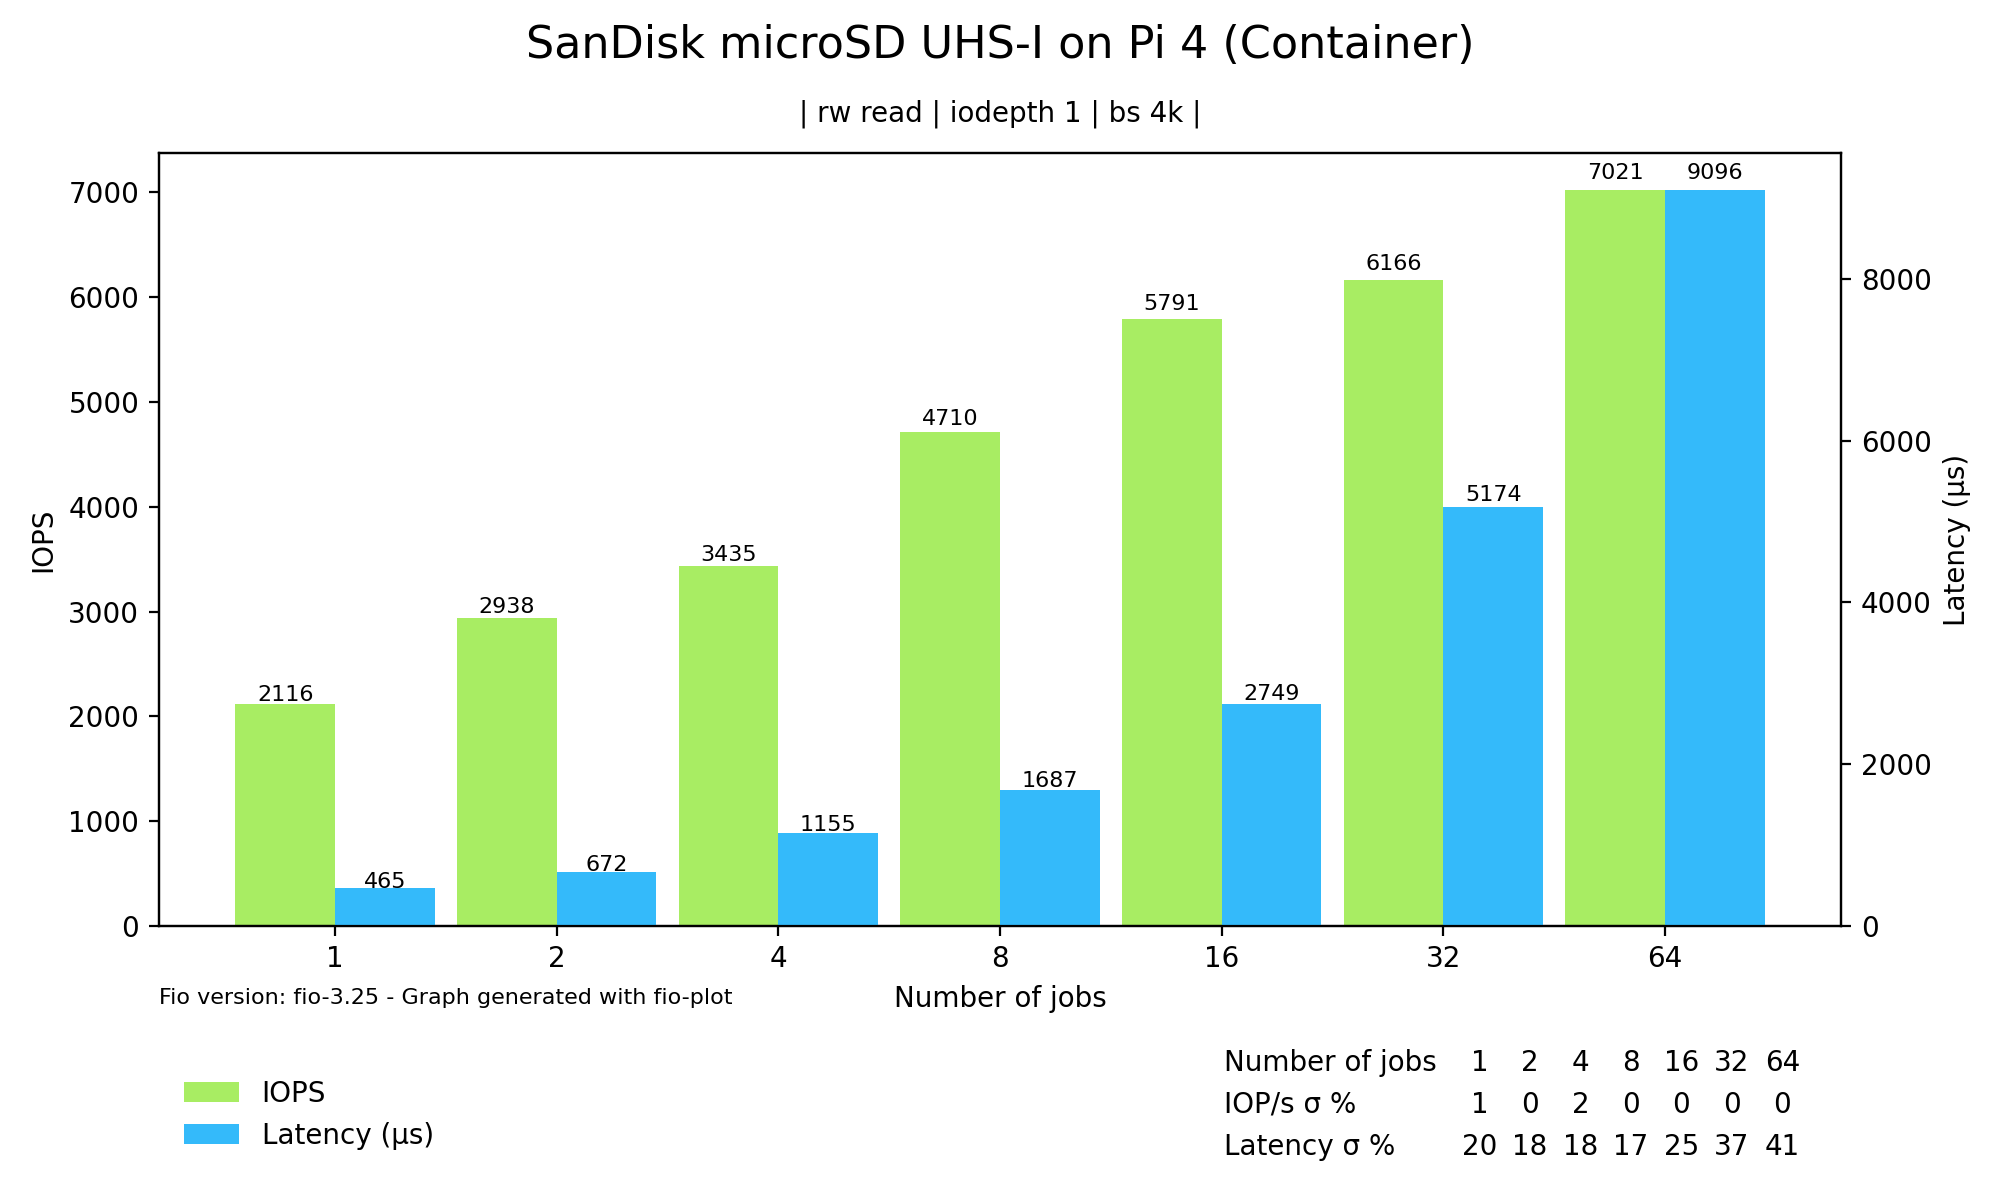
\includegraphics[width=0.8\textwidth]{images/results/sandisk-libaio-read-numjobs-iops-latency.png}
    \caption{Throughput and latency measurements within a container as a function of the number of concurrent processes issuing asynchronous reads.}
    \label{images:fundamentals/net-ns-veth-arch.jpg}
\end{figure}

\begin{figure}[H]
    \centering
    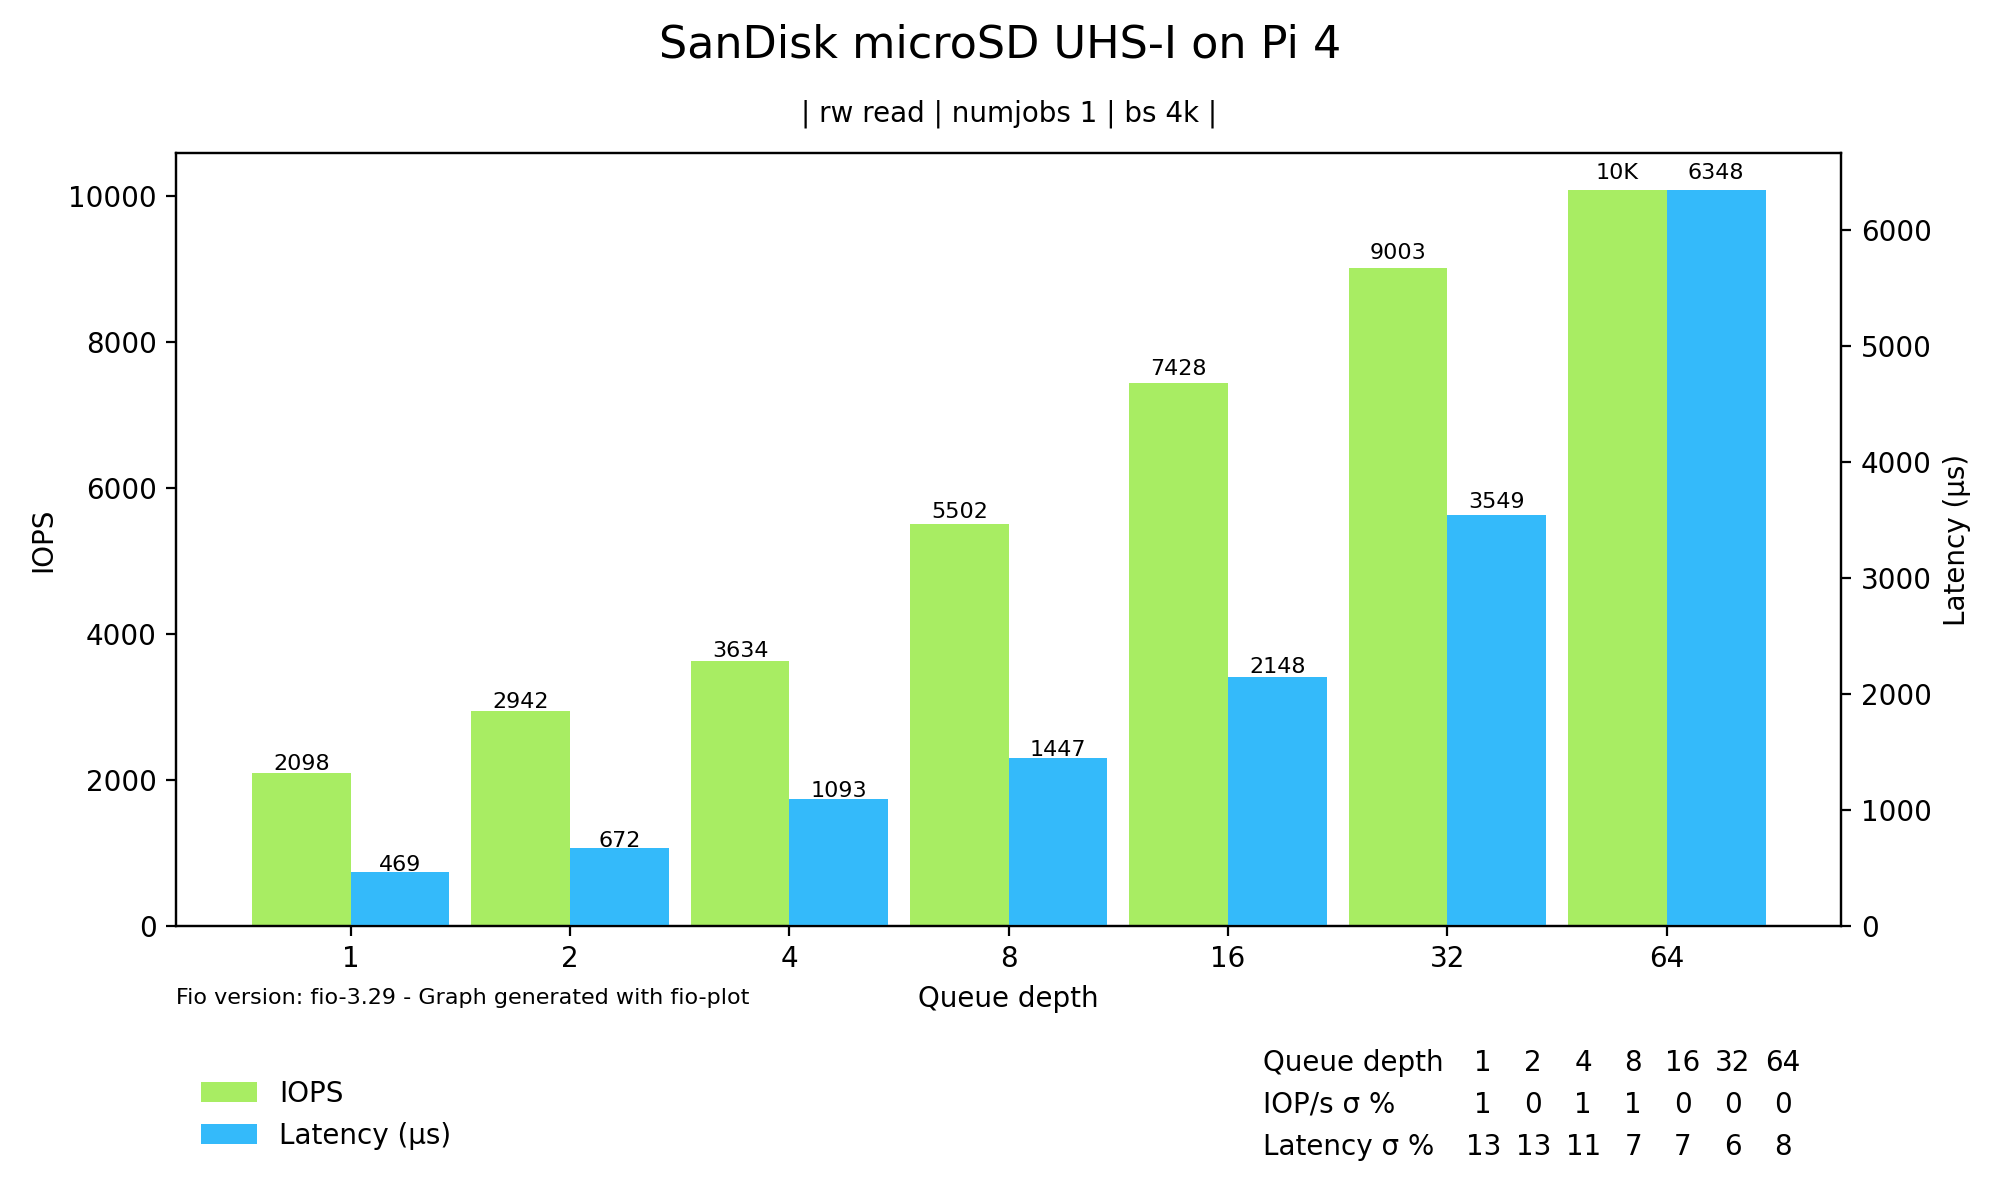
\includegraphics[width=0.8\textwidth]{images/results/sandisk-host-libaio-read-queue-depth-iops-latency.png}
    \caption{Throughput and latency measurements on the host as a function of the transmission queue length holding requests for asynchronous reads.}
    \label{images:fundamentals/net-ns-veth-arch.jpg}
\end{figure}

\begin{figure}[H]
    \centering
    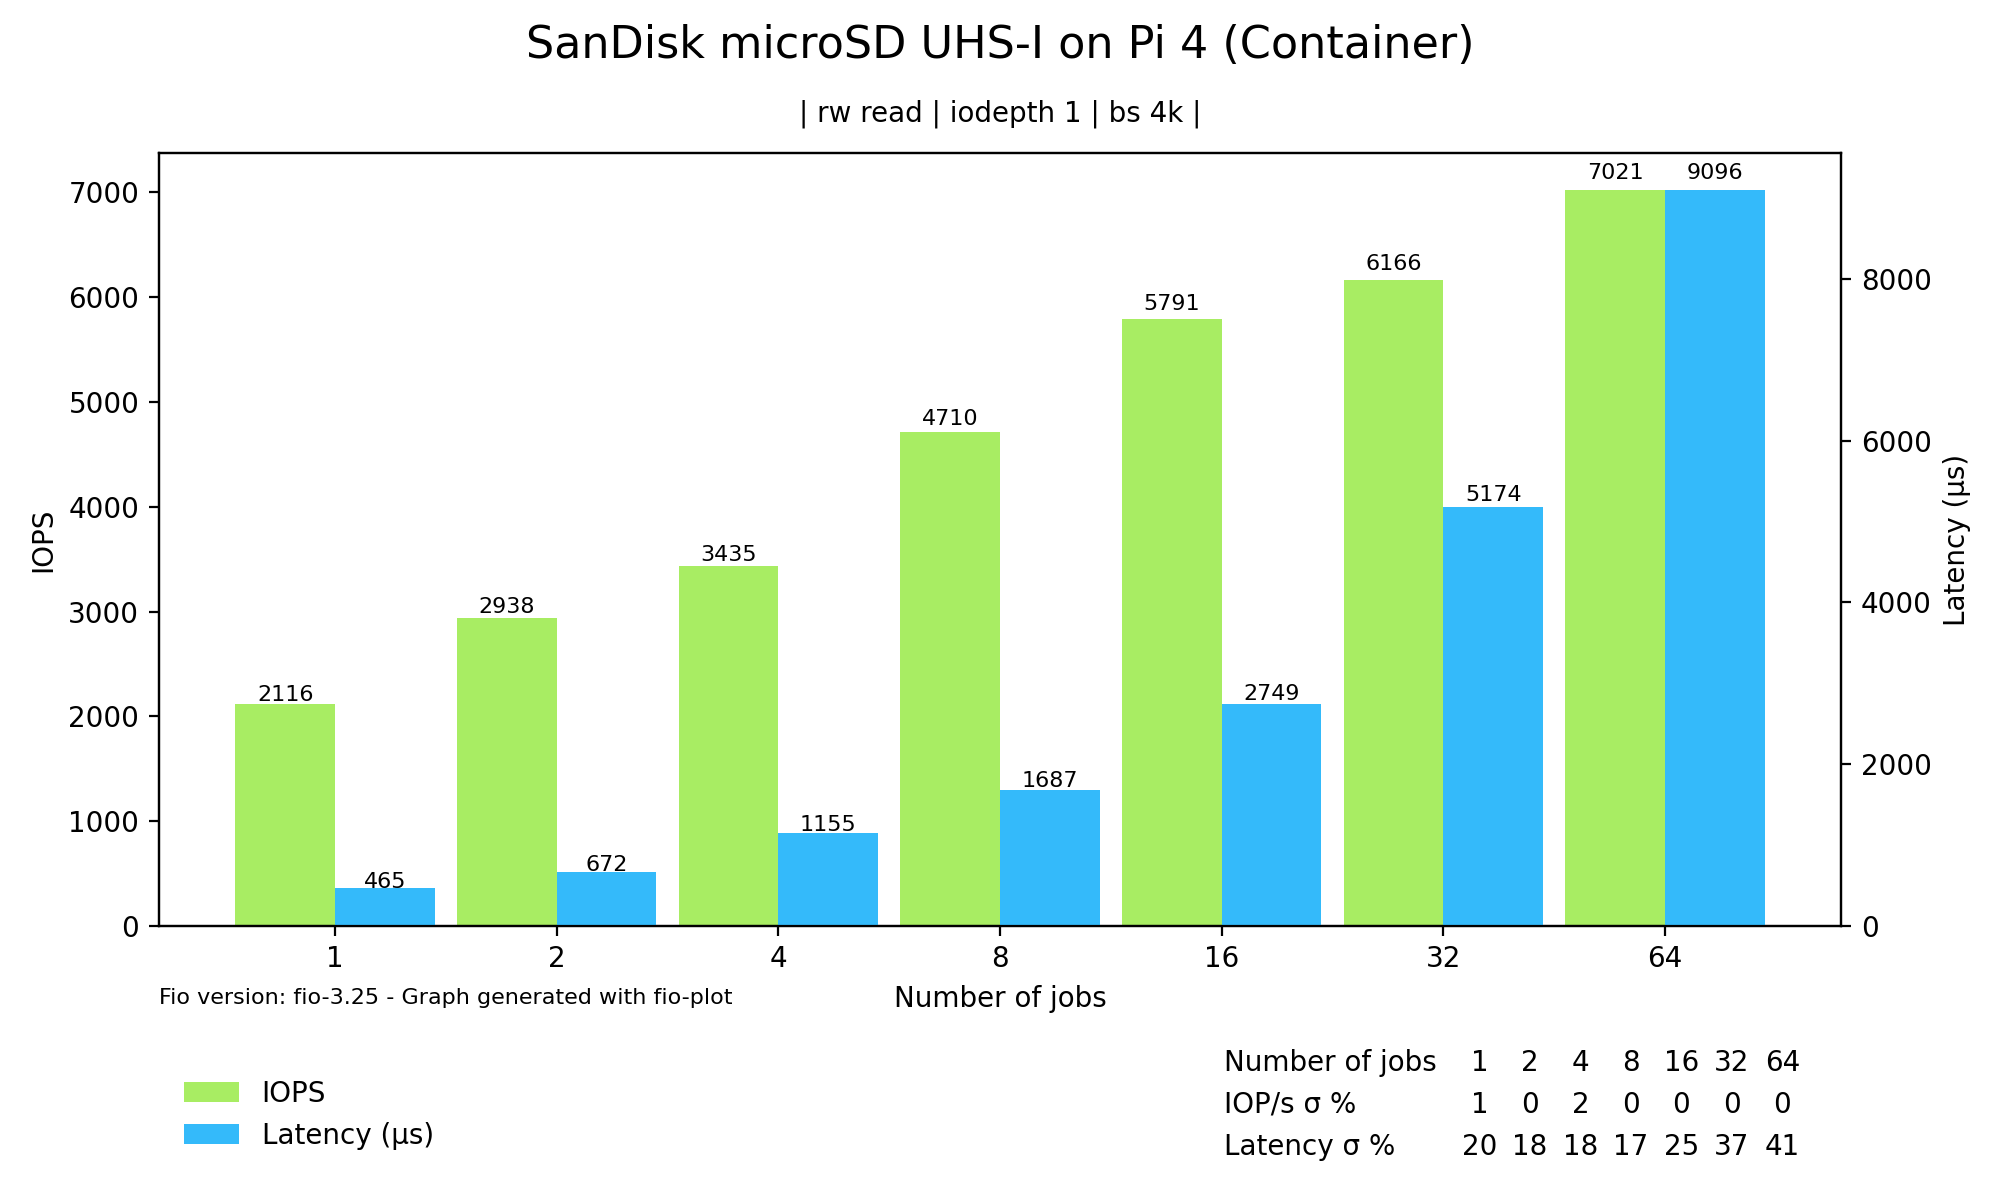
\includegraphics[width=0.8\textwidth]{images/results/sandisk-libaio-read-numjobs-iops-latency.png}
    \caption{Throughput and latency measurements within a container as a function of the transmission queue length holding requests for asynchronous reads.}
    \label{images:fundamentals/net-ns-veth-arch.jpg}
\end{figure}

\begin{figure}[H]
    \centering
    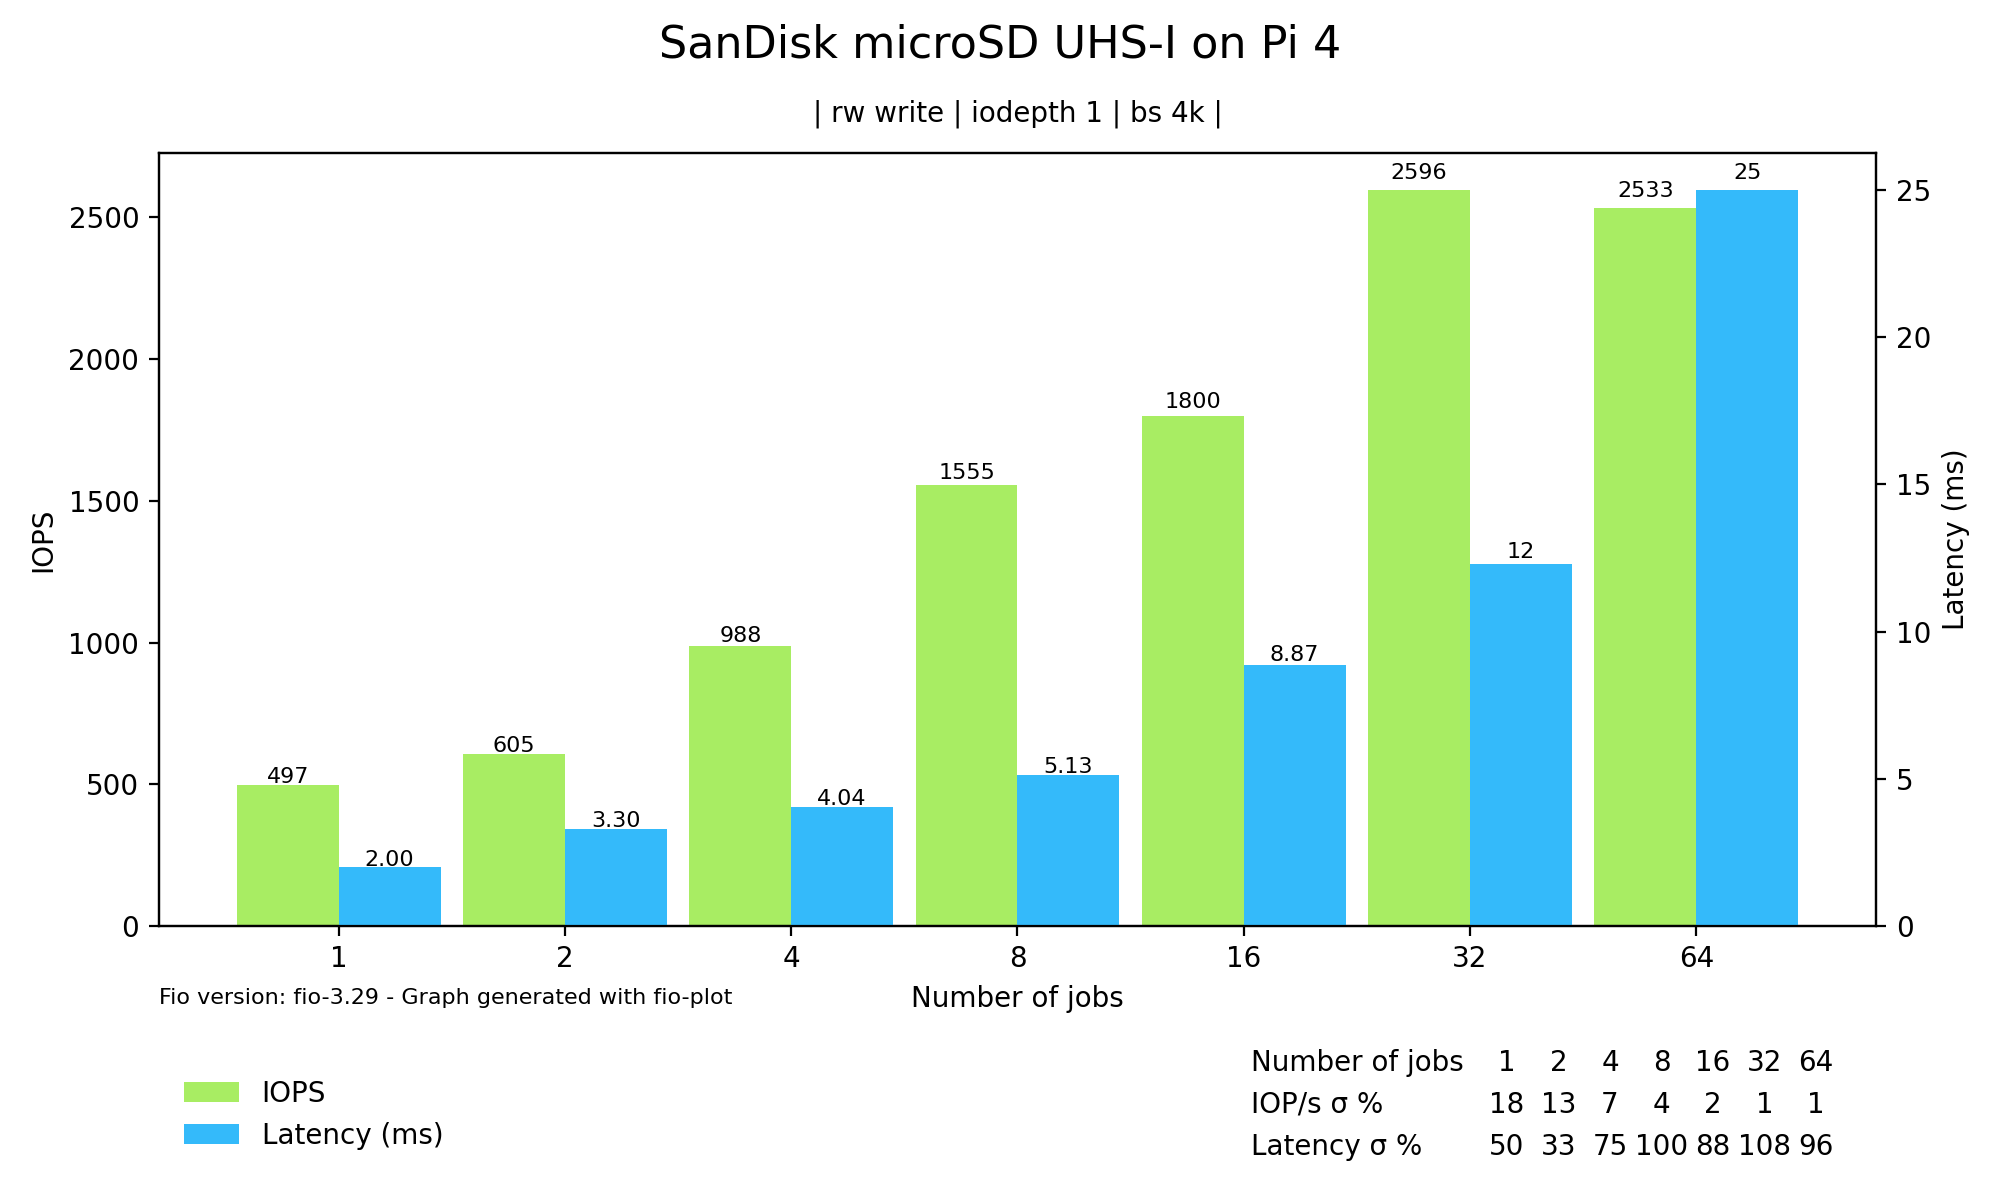
\includegraphics[width=0.8\textwidth]{images/results/sandisk-host-libaio-write-numjobs-iops-latency.png}
    \caption{Throughput and latency measurements on the host as a function of the number of concurrent processes issuing asynchronous writes.}
    \label{images:fundamentals/net-ns-veth-arch.jpg}
\end{figure}

\begin{figure}[H]
    \centering
    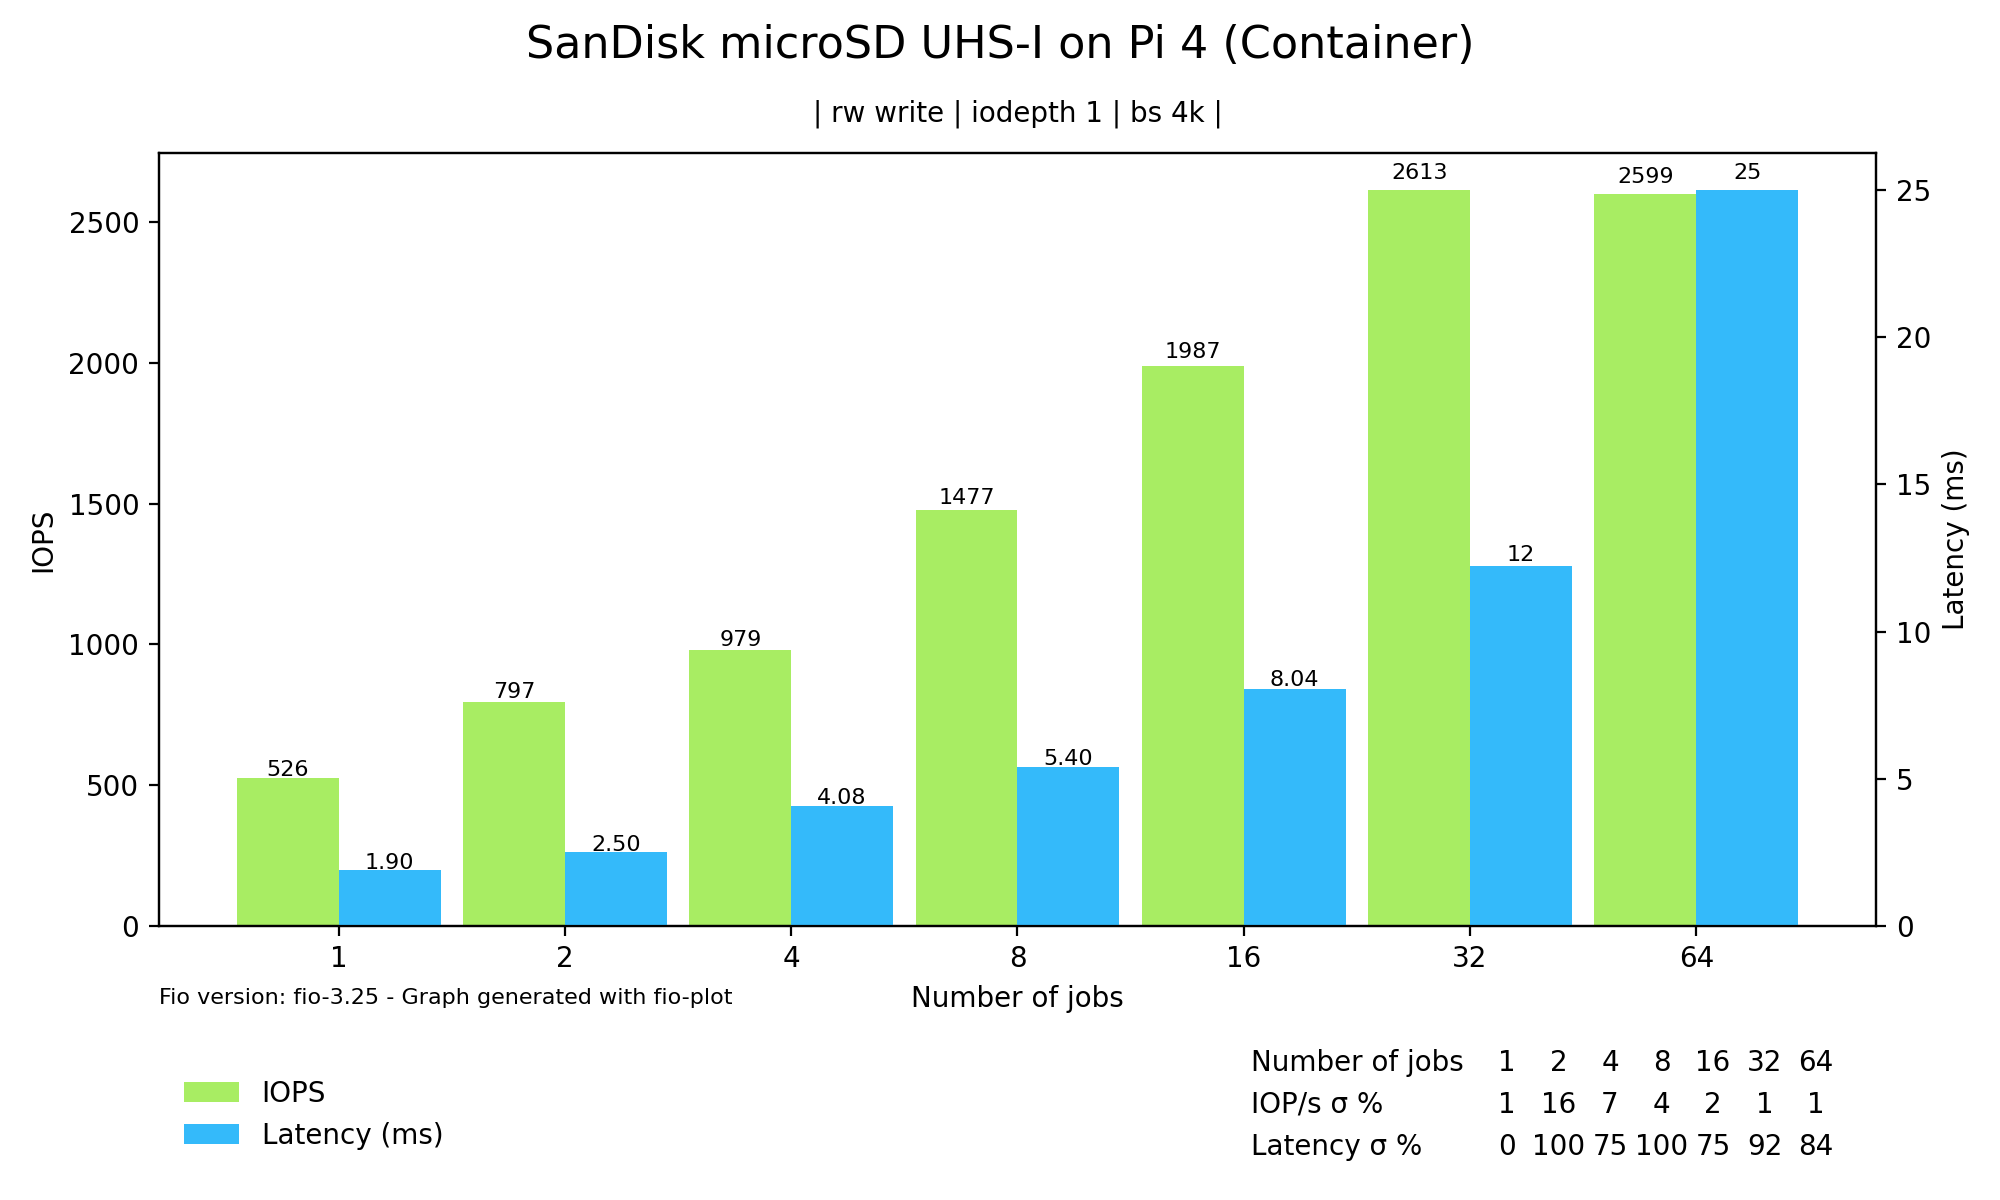
\includegraphics[width=0.8\textwidth]{images/results/sandisk-libaio-write-num-jobs-iops-latency.png}
    \caption{Asynchronous write latency and read throughput measured as a function of the number of concurrent processes inside a container}
    \label{images:fundamentals/net-ns-veth-arch.jpg}
\end{figure}

\begin{figure}[H]
    \centering
    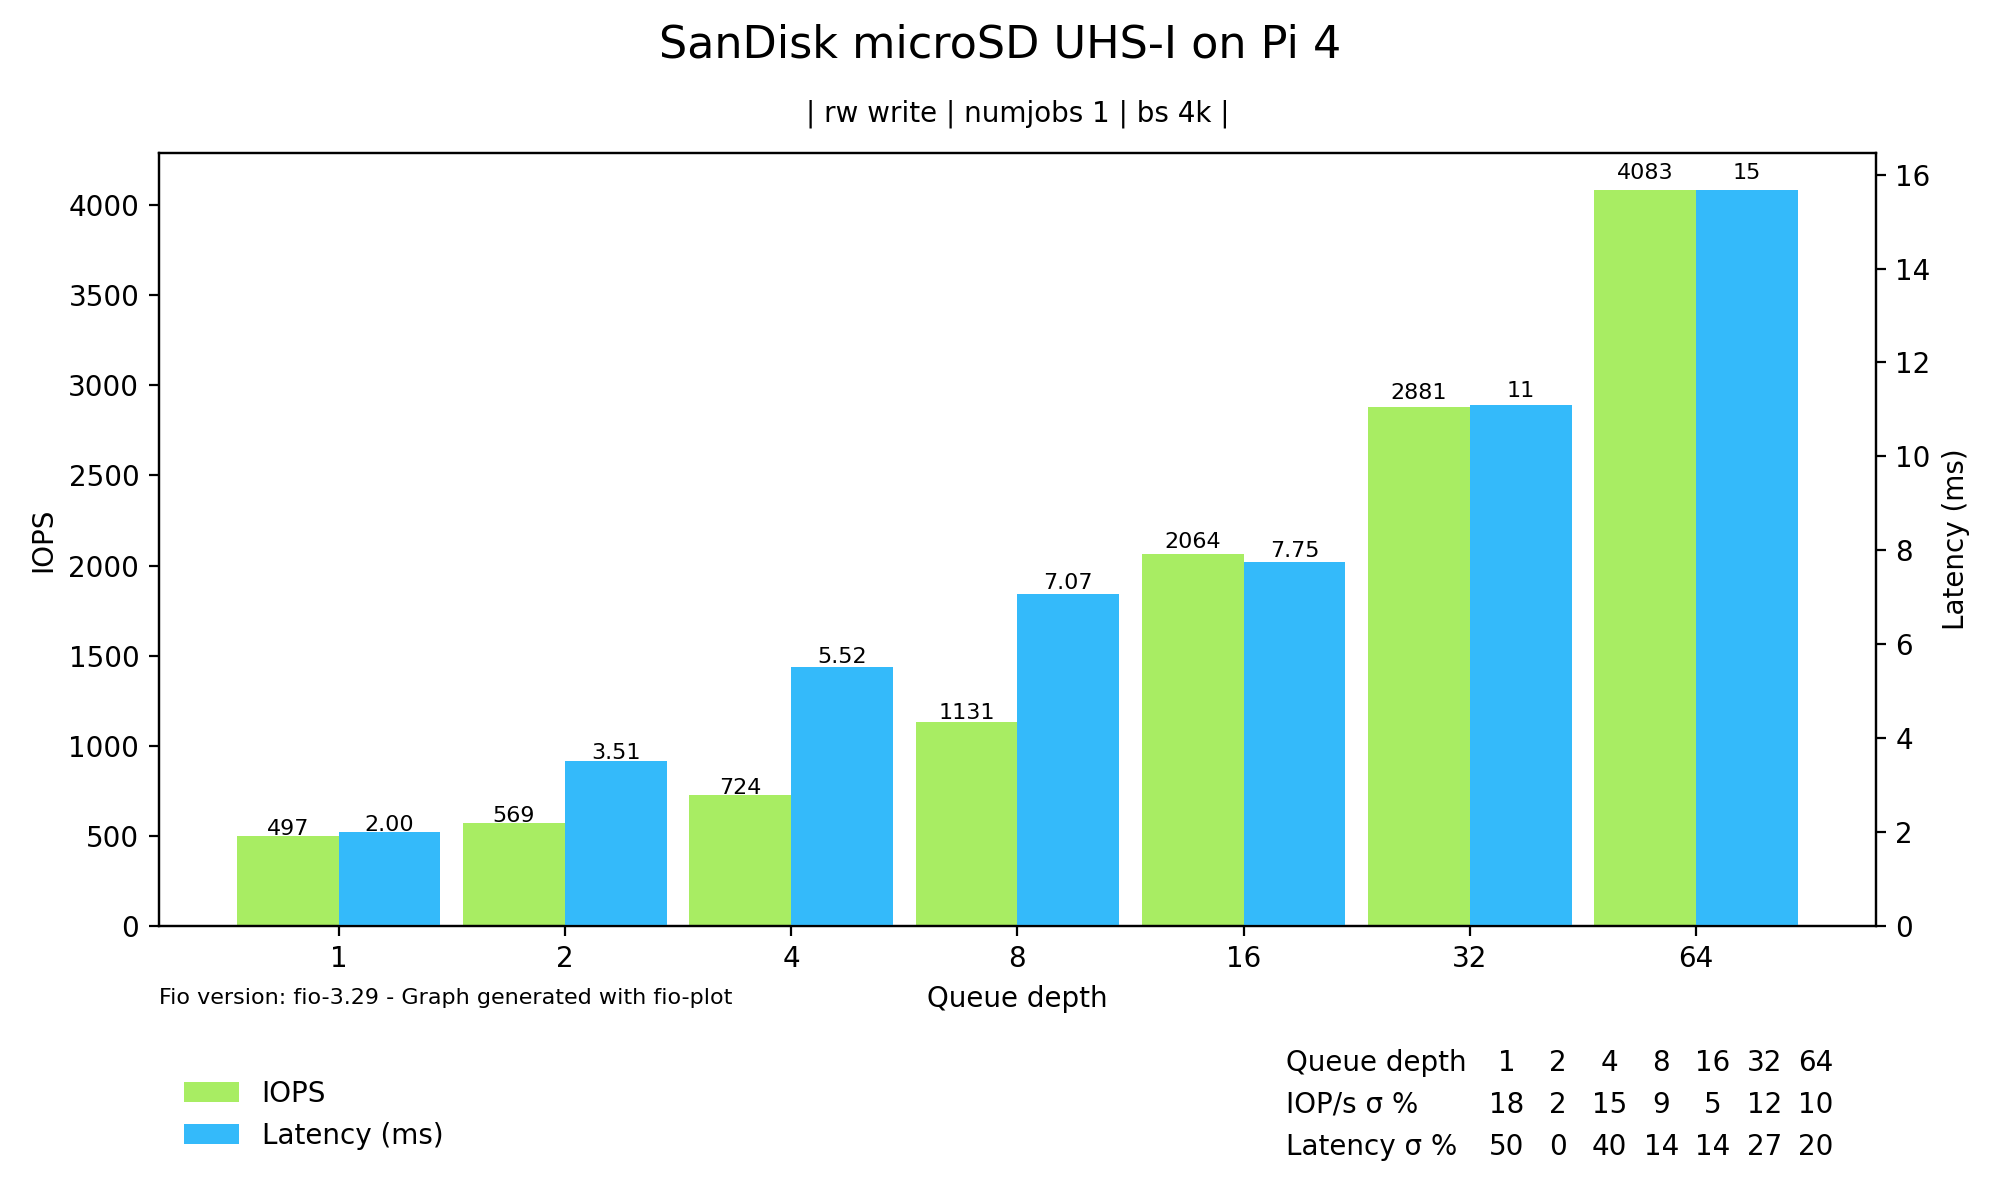
\includegraphics[width=0.8\textwidth]{images/results/sandisk-host-libaio-write-queue-depth-iops-latency.png}
    \caption{Throughput and latency measurements on the host as a function of the transmission queue length holding requests for asynchronous writes.}
    \label{images:fundamentals/net-ns-veth-arch.jpg}
\end{figure}

\begin{figure}[H]
    \centering
    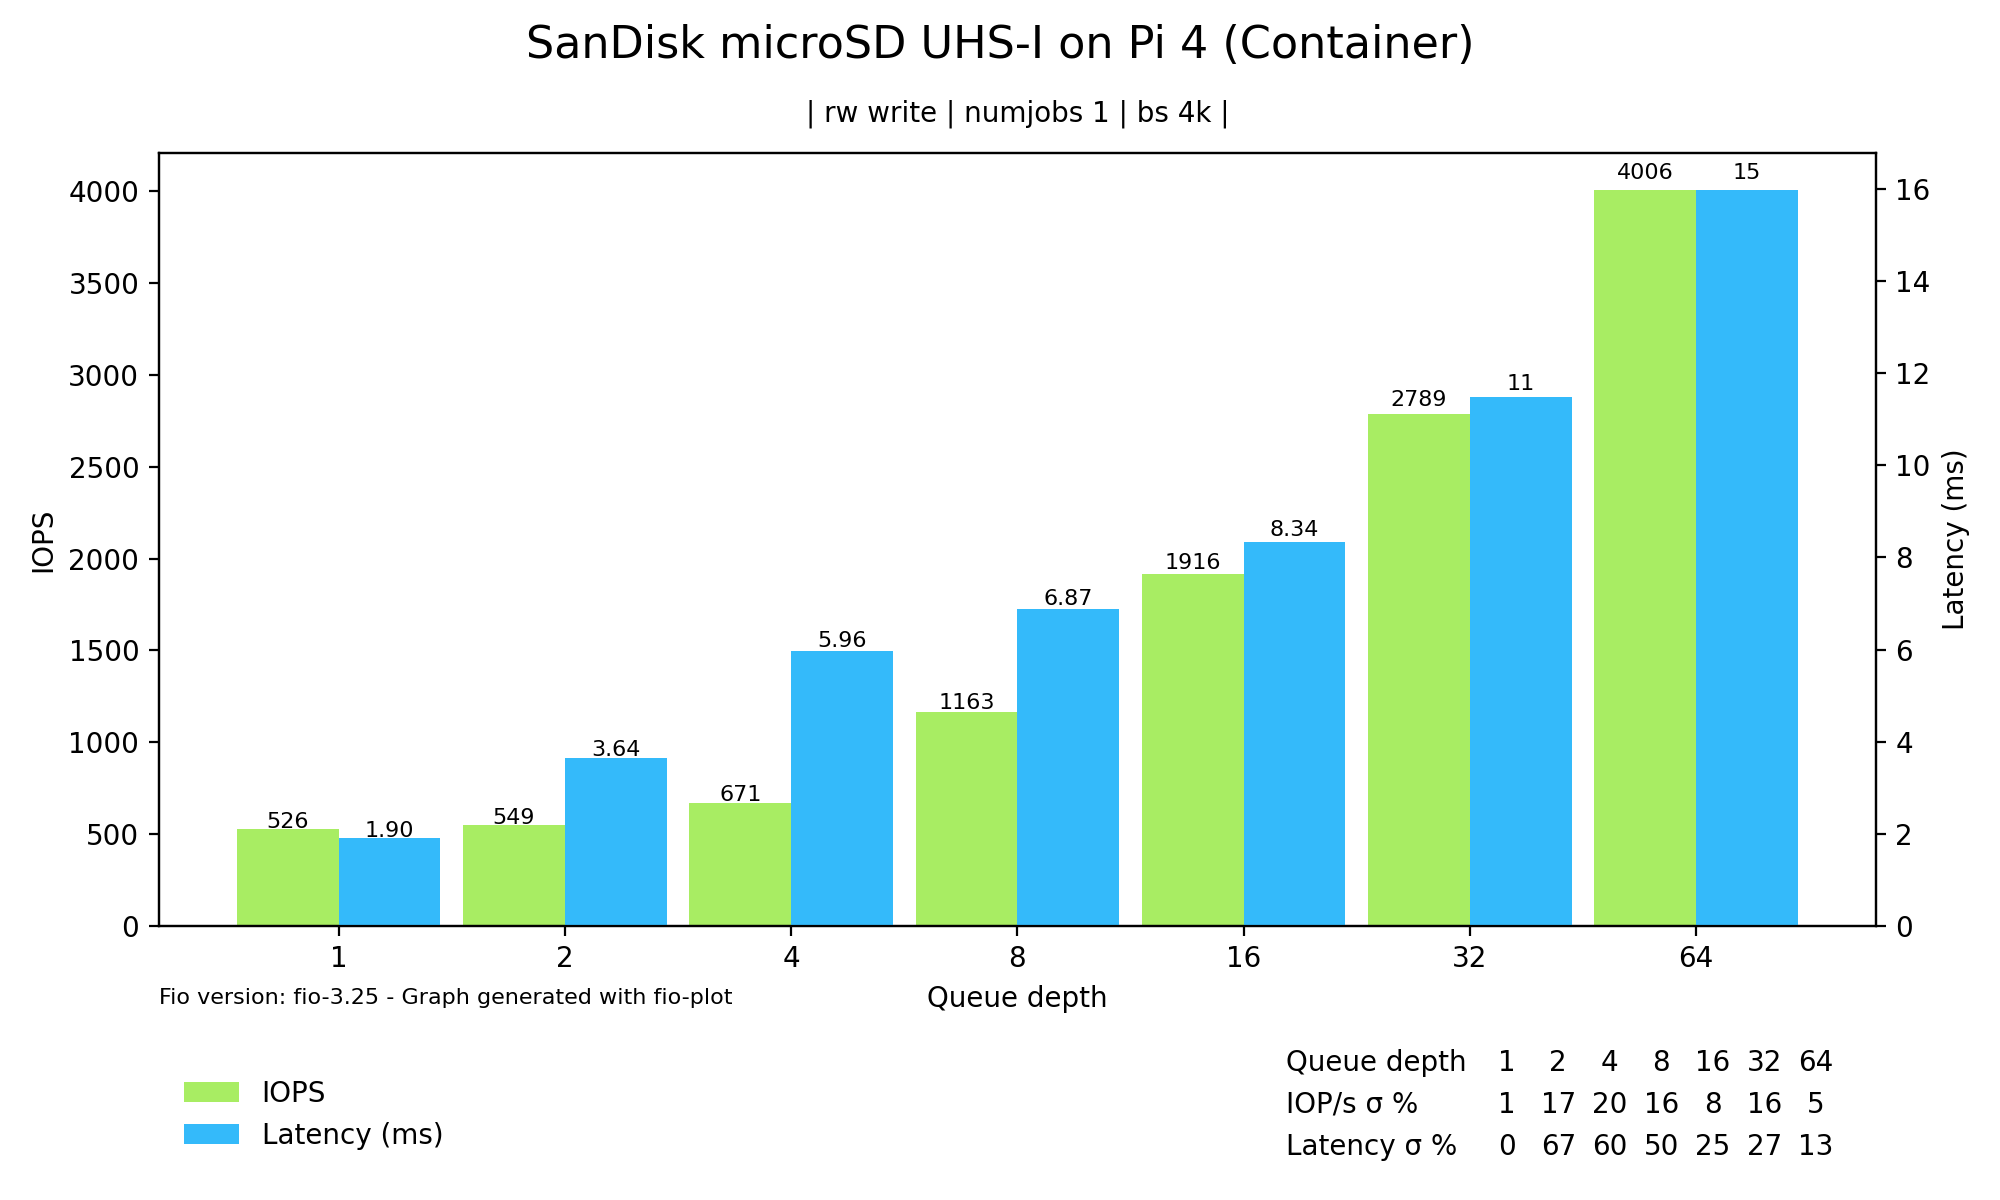
\includegraphics[width=0.8\textwidth]{images/results/sandisk-libaio-write-queue-depth-iops-latency.png}
    \caption{Throughput and latency measurements witihn a container as a function of the transmission queue length holding requests for asynchronous writes.}
    \label{images:fundamentals/net-ns-veth-arch.jpg}
\end{figure}


\begin{figure}[H]
    \centering
    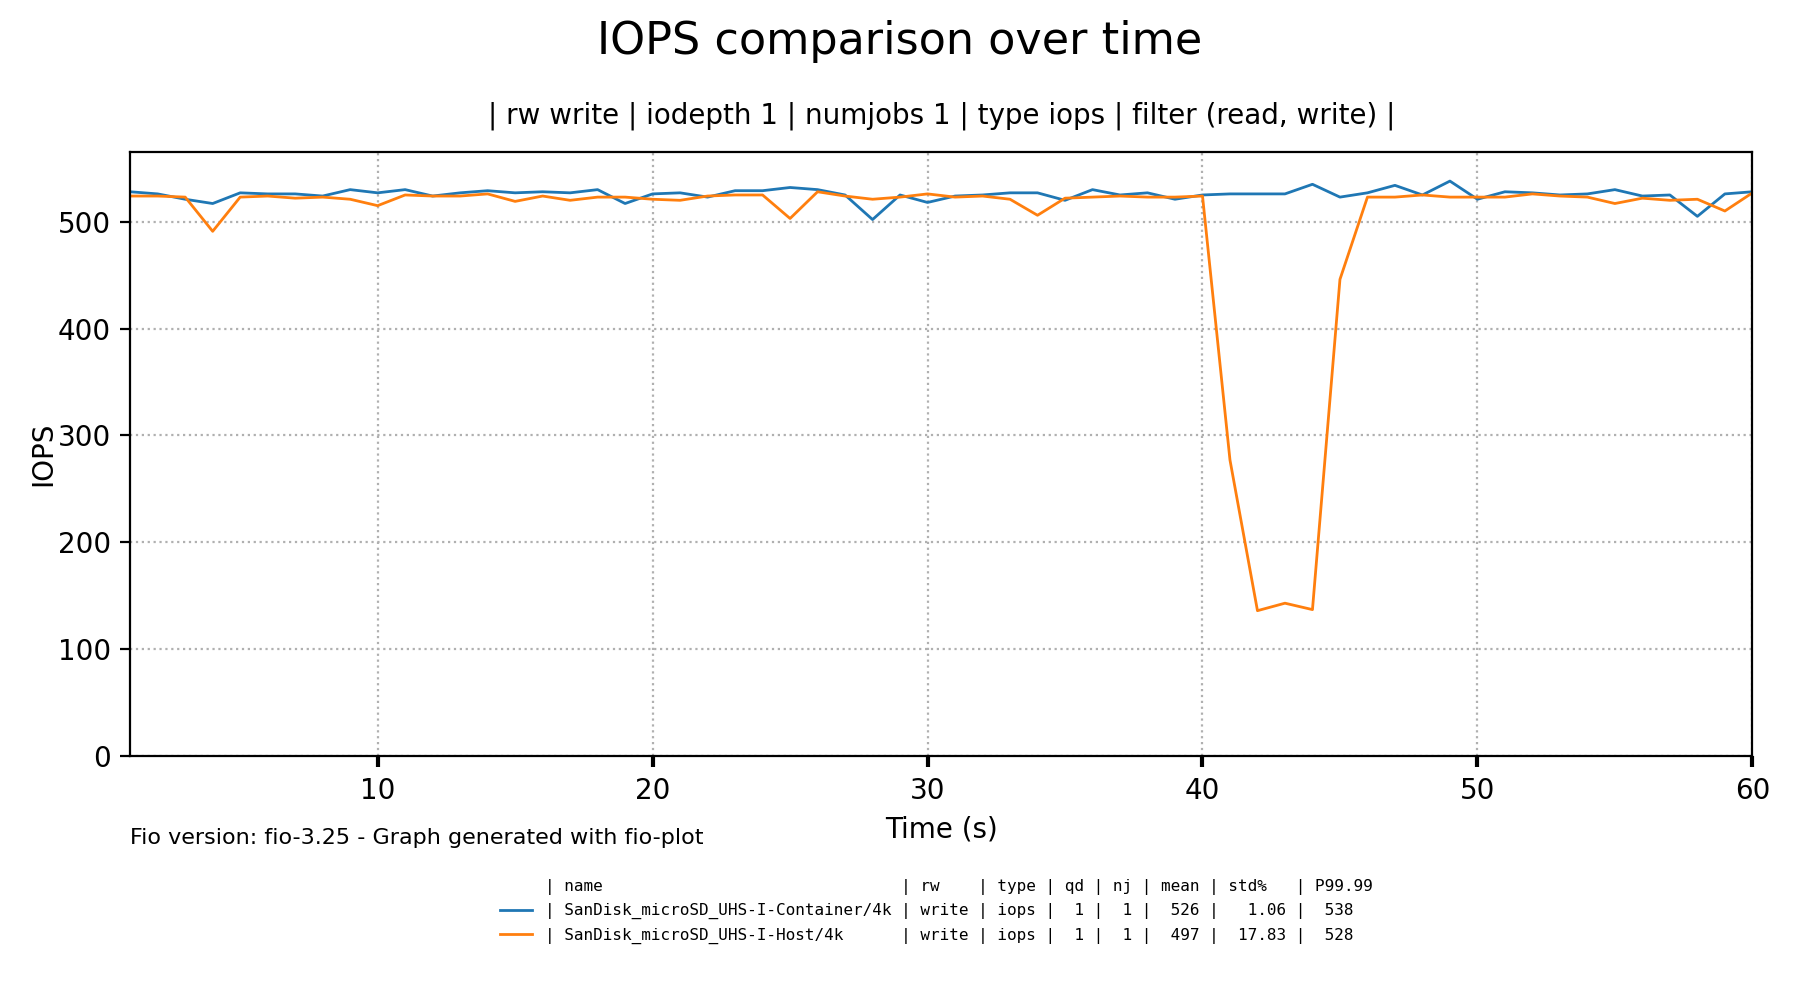
\includegraphics[width=0.8\textwidth]{images/results/sandisk-libaio-iops-write-comparison.png}
    \caption{Asynchronous write throughput on the host and inside a container, compared over time}
    \label{images:fundamentals/net-ns-veth-arch.jpg}
\end{figure}

\begin{figure}[H]
    \centering
    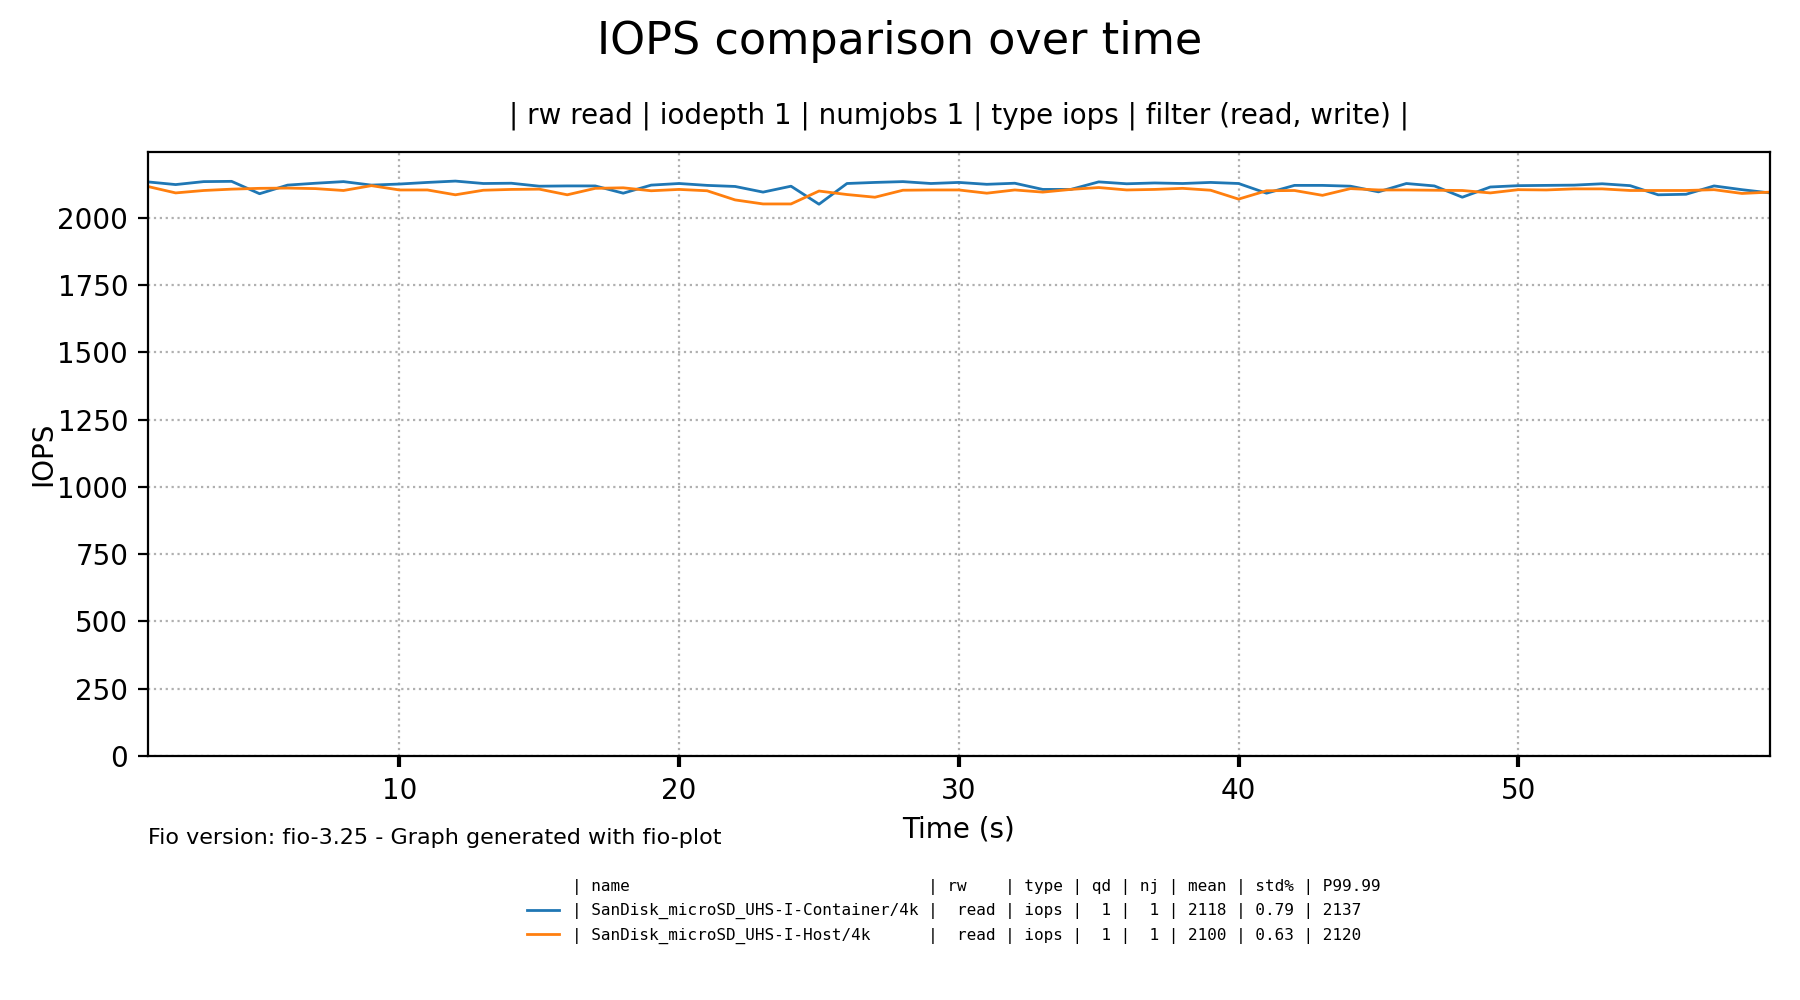
\includegraphics[width=0.8\textwidth]{images/results/sandisk-libaio-iops-read-comparison.png}
    \caption{Asynchronous read throughput on the host and inside a container, compared over time}
    \label{images:fundamentals/net-ns-veth-arch.jpg}
\end{figure}

\section{Network}
\label{ch:experiment/network}

\begin{figure}[H]
    \centering
    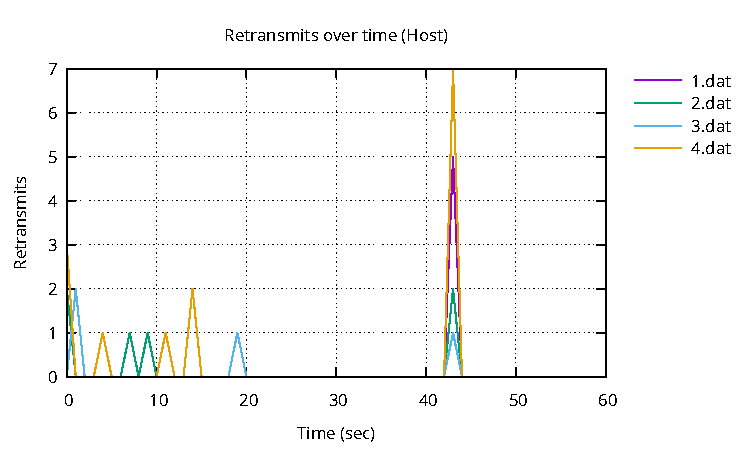
\includegraphics[width=1\textwidth]{images/results/network-host-retransmits.pdf}
    \caption{Number of packet retransmissions plotted over time on the host}
    \label{ticket-builder-class}
\end{figure}

\begin{figure}[H]
    \centering
    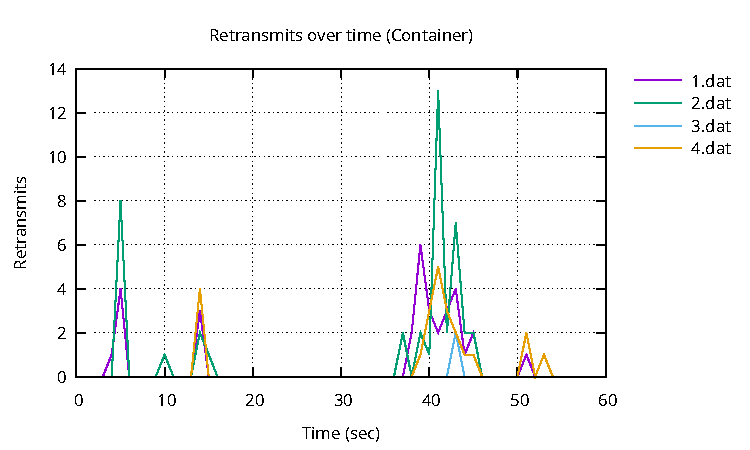
\includegraphics[width=1\textwidth]{images/results/network-retransmits-container.pdf}
    \caption{Number of packet retransmissions plotted over time within a container}
    \label{ticket-builder-class}
\end{figure}

\begin{figure}[H]
    \centering
    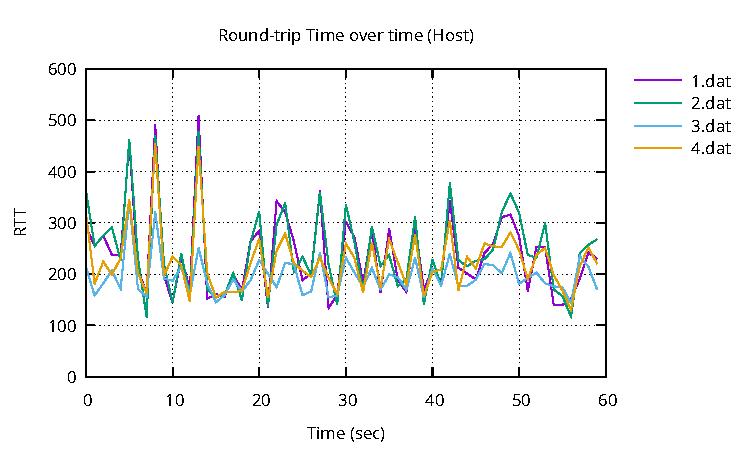
\includegraphics[width=1\textwidth]{images/results/network-host-rtt.pdf}
    \caption{Network latency (round-trip time) measured over time on the host}
    \label{ticket-builder-class}
\end{figure}

\begin{figure}[H]
    \centering
    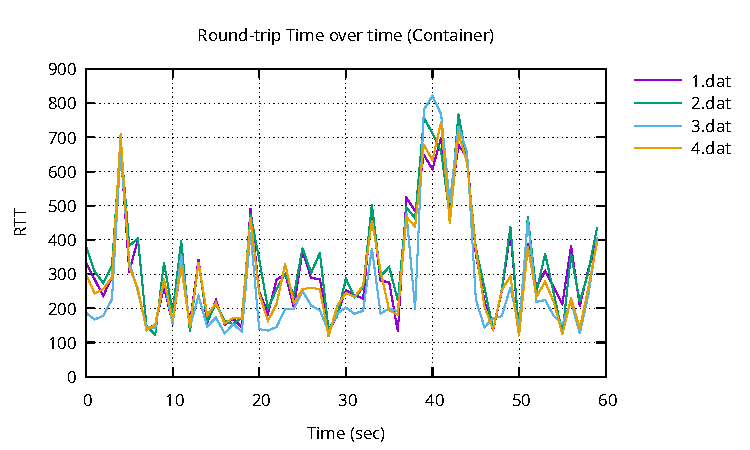
\includegraphics[width=1\textwidth]{images/results/network-rtt-container.pdf}
    \caption{Network latency (round-trip time) measured over time within a container}
    \label{ticket-builder-class}
\end{figure}

\begin{figure}[H]
    \centering
    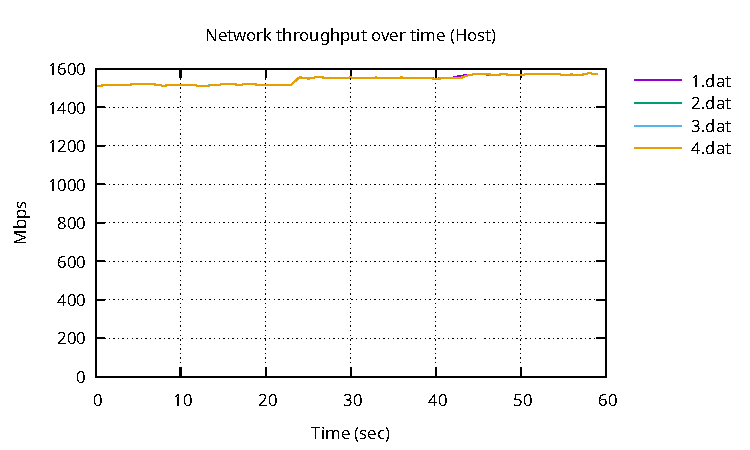
\includegraphics[width=1\textwidth]{images/results/network-host-throughput.pdf}
    \caption{Network throughput measured as megabits per second over time on the host}
    \label{ticket-builder-class}
\end{figure}

\begin{figure}[H]
    \centering
    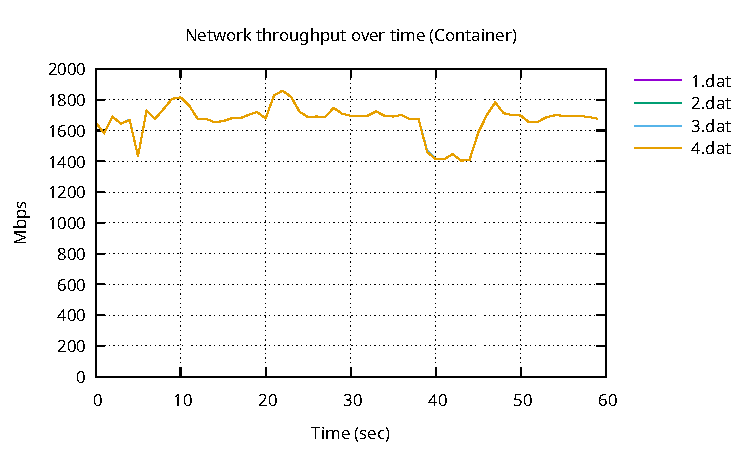
\includegraphics[width=1\textwidth]{images/results/network-throughput-container.pdf}
    \caption{Network throughput measured as megabits per second over time within a container}
    \label{ticket-builder-class}
\end{figure}